This section traces one refinement instance end to end, using the KNighter-derived CSA checker for Linux commit \texttt{97cba232549b}, which repairs an off-by-one access in the AMD display driver~\cite{linuxCommit97cba232,yang2025knighter}.
The case is small enough to inspect manually yet exhibits the core problem.
The generated checker recognizes a look-ahead access but misses the relation between the loop bound and the array's capacity.

\textbf{The bug and its patch.}
The member \lstinline|dc->links| has declared capacity \lstinline|MAX_PIPES * 2|, abbreviated as $N$ in Figure~\ref{fig:motivating} (\cmark{1}).
The function \lstinline|get_host_router_total_dp_tunnel_bw| iterates over candidate links.
On a matching host-router branch, it reads both \lstinline|links[i]| and \lstinline|links[i + 1]| (M10--M11, \cmark{3}).
With the original condition $i<N$ (M5, \cmark{2}), the loop permits $i=N-1$, so the look-ahead can reach index $N$, outside the array.
The patch changes the bound to $i<N-1$ (M6, \cmark{4}), limiting the largest look-ahead index to $N-1$.
Other branch conditions determine whether the access occurs; the new loop bound prevents this final out-of-range access.

\begin{figure}[!htbp]
  \centering
  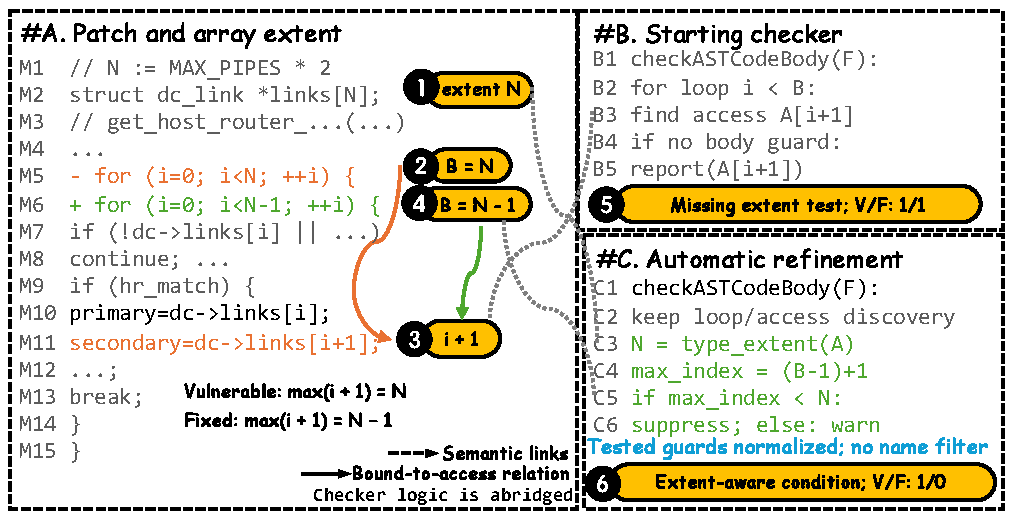
\includegraphics[width=0.70\textwidth]{figures/manual/motivating-example.pdf}
  \Description{A three-panel example. The left panel shows the array extent
  and the loop-bound patch. The upper-right panel shows the original
  look-ahead checker, which ignores the bound-to-capacity relation. The
  lower-right panel adds the maximum-index comparison while retaining the
  AST-based checker. Solid arrows relate loop bounds to the access; dashed arrows
  connect checker conditions to code.}
  \caption{\textbf{Capacity-aware look-ahead refinement.}
  Abridged code: $N$ denotes \lstinline|MAX_PIPES * 2| and
  \texttt{hr\_match} host-router equality. Independent vulnerable/fixed alerts
  change from \texttt{1/1} to \texttt{1/0}. This 14-response illustration used
  fixture feedback and differs from the one-response main-study checker.
  Orange/green arrows connect the bounds to the access; gray dotted links mark
  semantic correspondences.}
  \label{fig:motivating}
\end{figure}

\textbf{Why the baseline checker fails.}
The generated checker already recognizes an induction variable, a loop bound, and a look-ahead array subscript.
It reports an access when it does not recognize a protective condition in an enclosing \lstinline|if| (B1--B5, \cmark{5}).
That rule overlooks a guard carried by the loop condition itself.
The fixed program still contains \lstinline|links[i + 1]|, so the checker reports on both revisions despite the reduced loop bound.
Independent patch-related-object replay yields \texttt{1/1} alerts.
The checker has learned that a look-ahead access needs a guard, but not how the loop condition already supplies one.

\textbf{Evidence-guided refinement.}
\toolname starts from the same validation symptom and assembles the available patch, source and analyzer context.
This bundle has four provenance-labelled records: two internal Clang~18 CFG/call-graph records and two analyzer-output records.
The internal records anchor the loop and branch context to raw \texttt{debug.DumpCFG} and \texttt{debug.DumpCallGraph} output; patch and source context identify the bound change.

Both the starting and refined checkers use \lstinline|checkASTCodeBody|; the initial GLM-5.3-Flash edit adds a capacity-aware condition to the existing traversal.
The emitted checker reads the declared array extent from the AST type.
For the loop $i<B$, the maximum look-ahead index is $(B-1)+1=B$.
It suppresses the warning when that index is smaller than the known extent $N$ (C3--C6, \cmark{6}).
Thus the vulnerable $B=N$ remains reported, while the fixed $B=N-1$ becomes silent.
The condition uses type and index relations rather than the patched function name, a particular capacity, or adjacency of statements.
After two model calls, the candidate passes independent Linux replay at \texttt{1/0}.

\textbf{Checking the refinement.}
Further probes expose shortcomings in the candidate's fallback and inherited guard recognition.
Four automatic GPT-6-Luna-high quality continuations use 12 additional calls to repair these problems, giving 14 calls in total.
They receive the recorded fixture diagnostics; every scored checker edit is model-produced, and failed intermediate versions are retained.
The final checker still reports \texttt{1/0} on the Linux pair.
It passes 28 core fixtures, six boundary fixtures, 20 additional guard/bound fixtures, and 60 renamed/capacity-varied executions of those 20 forms: 58/58 unsafe and 56/56 safe executions overall.
AddressSanitizer also checks the labels of the latter 80 executions~\cite{serebryany2012asan}.

These tests cover name changes, unrelated statements, constant capacities and equivalent unit-step-loop/guard forms.
They informed the refinement, so they are a finite development suite rather than unseen-data confirmation or 114 independent bugs.
Arbitrary aliasing, dynamic extents and non-unit loop updates remain outside the tested forms.
The stronger illustration is kept separate from the 39-case experiment: its one-response G21 checker also reports \texttt{1/0} on the Linux pair but passes 74/114 of these fixtures.
Neither version isolates the contribution of internal records from the other supplied context.
